\tikzstyle{hidden_neuron}=[circle,draw=blue!50,fill=cyan!10,thick,minimum size=4mm]
\begin{tikzpicture}
\newcommand*{\xpos}{10}
\newcommand*{\ypos}{10}
\newcommand*{\rectstarty}{6}
\newcommand*{\rectendy}{6.5}


%%%%%%%%%%%%%%Generator

% Generator
\visible<6->
{
	\renewcommand*{\xpos}{20}
	\draw[rounded corners,fill=green!12] (\xpos-0.5, \rectstarty+1) rectangle (\xpos+2, \rectendy+1) {};
	\node (N) at (\xpos+0.75,\rectendy+0.75) {\small{Generator}};

	% Sample z
	\draw[rounded corners,fill=cyan!20] (\xpos-0.5, \rectstarty) rectangle (\xpos+2, \rectendy) {};
	\node[hidden_neuron] (N1) at (\xpos,\rectstarty+0.25) {};
	\node[hidden_neuron] (N2) at (\xpos+1*0.5,\rectstarty+0.25) {};
	\node[hidden_neuron] (N3) at (\xpos+2*0.5,\rectstarty+0.25) {};
	\node[hidden_neuron] (N4) at (\xpos+3*0.5,\rectstarty+0.25) {};
	\node (N) at (\xpos+1,\rectstarty-0.5) {\small{$z \sim N(0,I)$}};

	% Bottom arrow
	\draw[->,thick,black] (\xpos+0.75,\rectendy) -- (\xpos+0.75,\rectendy+0.5);

	% Images
	\node (N) at (\xpos+0.75,\rectstarty+2.2) {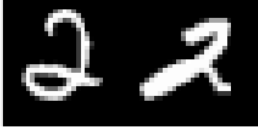
\includegraphics[scale=0.1]{images/two_gen.png}};

	% Top arrow
	\draw[->,thick,black] (\xpos+0.75,\rectendy+1) -- (\xpos+0.75,\rectendy+1.5);
}
%%%%%%%%%%%%%%%Real world images
\visible<8->
{
	\renewcommand*{\xpos}{23}

	% Real Images
	\draw[rounded corners,fill=green!12] (\xpos-0.5, \rectstarty+1) rectangle (\xpos+2, \rectendy+1) {};
	\node (N) at (\xpos+0.75,\rectendy+0.75) {\small{Real Images}};

	% Images
	\node (N) at (\xpos+0.75,\rectstarty+2.2) {
\includegraphics[scale=0.1]{images/two_real.png}};

	% Top arrow
	\draw[->,thick,black] (\xpos+0.75,\rectendy+1) -- (\xpos+0.75,\rectendy+1.5);

	\renewcommand*{\xpos}{23}
	\draw[->,thick,black] (\xpos+0.75,\rectendy+1.9) -- (\xpos+0.75-0.7,\rectstarty+3);
}
%%%%%%%%%%%%%%%% Discriminator
\visible<7->
{
	\renewcommand*{\xpos}{21.5}
	% Discriminator
	\draw[rounded corners,fill=green!12] (\xpos-0.5, \rectstarty+3) rectangle (\xpos+2, \rectendy+3) {};
	\node (N) at (\xpos+0.75,\rectendy+2.75) {\small{Discriminator	}};
	\visible<9->
	{
		\draw[->,thick,black] (\xpos+0.75,\rectendy+3) -- (\xpos+0.75,\rectendy+3.4);
		\node (N) at (\xpos+0.75,\rectendy+3.52) {\small {Real or Fake}};
	}

	% Arrows
	\renewcommand*{\xpos}{20}
	\draw[->,thick,black] (\xpos+0.75,\rectendy+1.9) -- (\xpos+0.75+0.7,\rectstarty+3);
}
\end{tikzpicture}